\documentclass{standalone}
\usepackage{tikz}
\usetikzlibrary{patterns, positioning}


\begin{document}
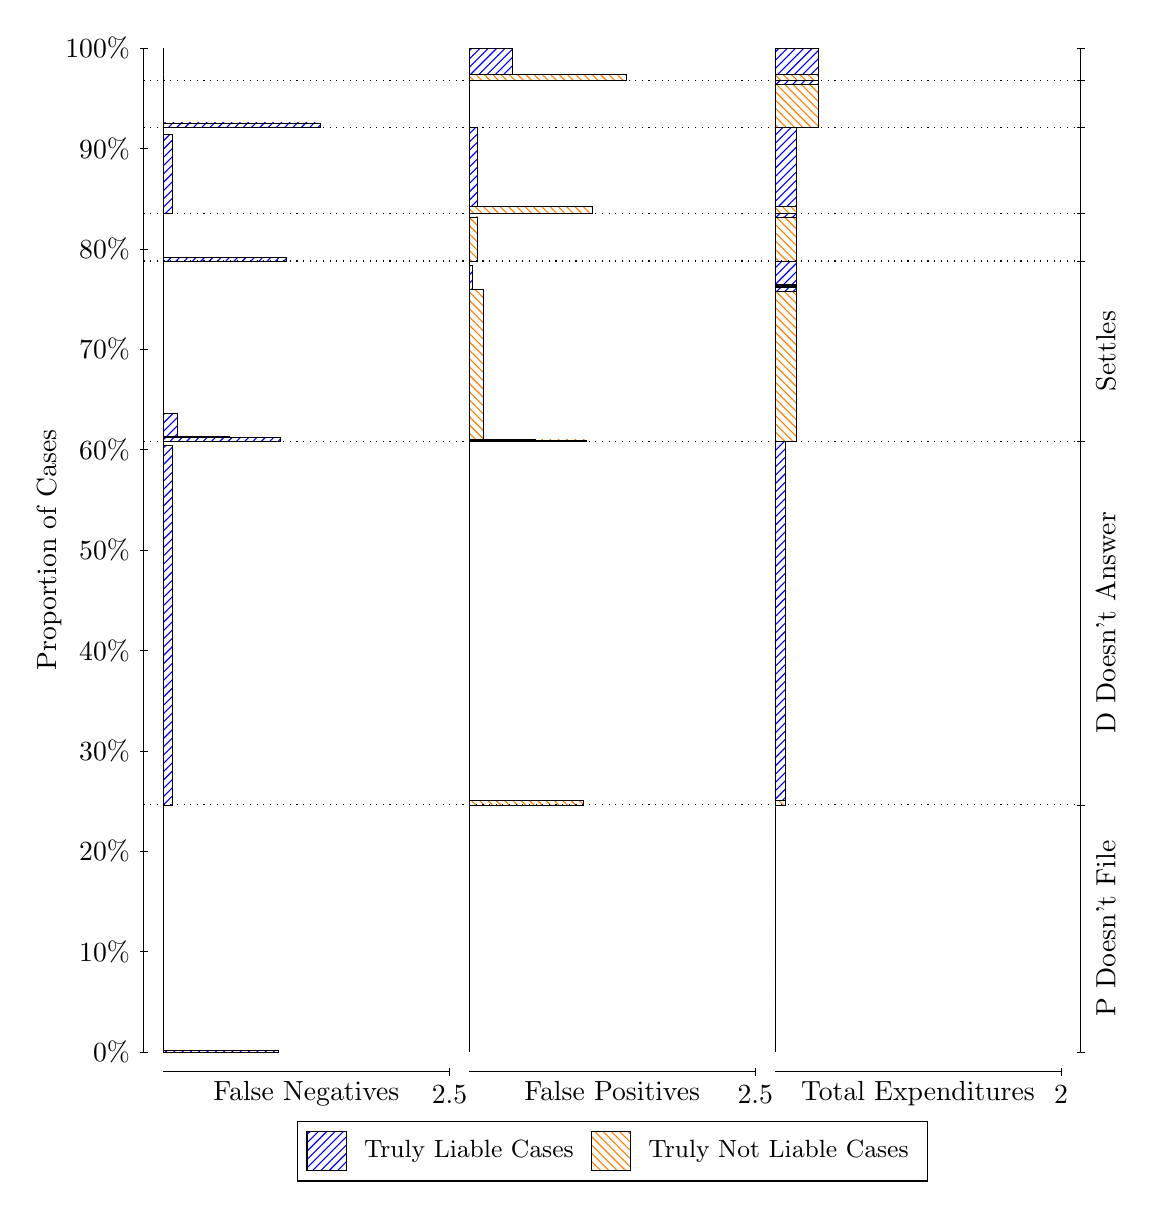
\begin{tikzpicture}
\draw[black, very thin] (1.5,1.75) -- (1.5,14.5);
\node[rotate=90, text=black, anchor=center] at (0.3, 8.125) {Proportion of Cases};
\draw[black, very thin] (1.45,1.75) -- (1.55,1.75);
\node[text=black, anchor=east] at (1.45, 1.75) {0\%};
\draw[black, very thin] (1.45,3.025) -- (1.55,3.025);
\node[text=black, anchor=east] at (1.45, 3.025) {10\%};
\draw[black, very thin] (1.45,4.3) -- (1.55,4.3);
\node[text=black, anchor=east] at (1.45, 4.3) {20\%};
\draw[black, very thin] (1.45,5.575) -- (1.55,5.575);
\node[text=black, anchor=east] at (1.45, 5.575) {30\%};
\draw[black, very thin] (1.45,6.85) -- (1.55,6.85);
\node[text=black, anchor=east] at (1.45, 6.85) {40\%};
\draw[black, very thin] (1.45,8.125) -- (1.55,8.125);
\node[text=black, anchor=east] at (1.45, 8.125) {50\%};
\draw[black, very thin] (1.45,9.4) -- (1.55,9.4);
\node[text=black, anchor=east] at (1.45, 9.4) {60\%};
\draw[black, very thin] (1.45,10.675) -- (1.55,10.675);
\node[text=black, anchor=east] at (1.45, 10.675) {70\%};
\draw[black, very thin] (1.45,11.95) -- (1.55,11.95);
\node[text=black, anchor=east] at (1.45, 11.95) {80\%};
\draw[black, very thin] (1.45,13.225) -- (1.55,13.225);
\node[text=black, anchor=east] at (1.45, 13.225) {90\%};
\draw[black, very thin] (1.45,14.5) -- (1.55,14.5);
\node[text=black, anchor=east] at (1.45, 14.5) {100\%};

\draw[black, very thin] (13.4,1.75) -- (13.4,14.5);
\draw[black, very thin] (13.35,1.75) -- (13.45,1.75);
\node[anchor=west] at (13.35, 1.75) {};
\draw[black, very thin] (13.35,4.8878) -- (13.45,4.8878);
\node[anchor=west] at (13.35, 4.8878) {};
\draw[black, very thin] (13.35,9.5079) -- (13.45,9.5079);
\node[anchor=west] at (13.35, 9.5079) {};
\draw[black, very thin] (13.35,11.795) -- (13.45,11.795);
\node[anchor=west] at (13.35, 11.795) {};
\draw[black, very thin] (13.35,12.4) -- (13.45,12.4);
\node[anchor=west] at (13.35, 12.4) {};
\draw[black, very thin] (13.35,13.492) -- (13.45,13.492);
\node[anchor=west] at (13.35, 13.492) {};
\draw[black, very thin] (13.35,14.091) -- (13.45,14.091);
\node[anchor=west] at (13.35, 14.091) {};
\draw[black, very thin] (13.35,14.5) -- (13.45,14.5);
\node[anchor=west] at (13.35, 14.5) {};

\draw[black, very thin, pattern color=blue, pattern=north east lines] (1.75,1.75) rectangle (3.2033,1.7676);
\draw[black, very thin, pattern color=orange, pattern=north west lines] (1.75,1.7676) rectangle (1.75,4.8878);
\draw[black, very thin, pattern color=blue, pattern=north east lines] (1.75,4.8878) rectangle (1.859,9.4526);
\draw[black, very thin, pattern color=orange, pattern=north west lines] (1.75,9.4526) rectangle (1.75,9.5079);
\draw[black, very thin, pattern color=blue, pattern=north east lines] (1.75,9.5079) rectangle (3.2397,9.5592);
\draw[black, very thin, pattern color=blue, pattern=north east lines] (1.75,9.5592) rectangle (2.5857,9.566);
\draw[black, very thin, pattern color=blue, pattern=north east lines] (1.75,9.566) rectangle (1.9317,9.863);
\draw[black, very thin, pattern color=orange, pattern=north west lines] (1.75,9.863) rectangle (1.75,11.795);
\draw[black, very thin, pattern color=blue, pattern=north east lines] (1.75,11.795) rectangle (3.3123,11.839);
\draw[black, very thin, pattern color=orange, pattern=north west lines] (1.75,11.839) rectangle (1.75,12.4);
\draw[black, very thin, pattern color=blue, pattern=north east lines] (1.75,12.4) rectangle (1.859,13.401);
\draw[black, very thin, pattern color=orange, pattern=north west lines] (1.75,13.401) rectangle (1.75,13.492);
\draw[black, very thin, pattern color=blue, pattern=north east lines] (1.75,13.492) rectangle (3.7483,13.548);
\draw[black, very thin, pattern color=orange, pattern=north west lines] (1.75,13.548) rectangle (1.75,14.091);
\draw[black, very thin, pattern color=orange, pattern=north west lines] (1.75,14.091) rectangle (1.75,14.166);
\draw[black, very thin, pattern color=blue, pattern=north east lines] (1.75,14.166) rectangle (1.75,14.5);
\draw[black, very thin, pattern color=orange, pattern=north west lines] (5.6333,1.75) rectangle (5.6333,4.8701);
\draw[black, very thin, pattern color=blue, pattern=north east lines] (5.6333,4.8701) rectangle (5.6333,4.8878);
\draw[black, very thin, pattern color=orange, pattern=north west lines] (5.6333,4.8878) rectangle (7.0867,4.9431);
\draw[black, very thin, pattern color=blue, pattern=north east lines] (5.6333,4.9431) rectangle (5.6333,9.5079);
\draw[black, very thin, pattern color=orange, pattern=north west lines] (5.6333,9.5079) rectangle (7.123,9.5222);
\draw[black, very thin, pattern color=orange, pattern=north west lines] (5.6333,9.5222) rectangle (6.469,9.5337);
\draw[black, very thin, pattern color=orange, pattern=north west lines] (5.6333,9.5337) rectangle (5.815,11.439);
\draw[black, very thin, pattern color=blue, pattern=north east lines] (5.6333,11.439) rectangle (5.6697,11.736);
\draw[black, very thin, pattern color=blue, pattern=north east lines] (5.6333,11.736) rectangle (5.6333,11.795);
\draw[black, very thin, pattern color=orange, pattern=north west lines] (5.6333,11.795) rectangle (5.7423,12.355);
\draw[black, very thin, pattern color=blue, pattern=north east lines] (5.6333,12.355) rectangle (5.6333,12.4);
\draw[black, very thin, pattern color=orange, pattern=north west lines] (5.6333,12.4) rectangle (7.1957,12.49);
\draw[black, very thin, pattern color=blue, pattern=north east lines] (5.6333,12.49) rectangle (5.7423,13.492);
\draw[black, very thin, pattern color=orange, pattern=north west lines] (5.6333,13.492) rectangle (5.6333,14.034);
\draw[black, very thin, pattern color=blue, pattern=north east lines] (5.6333,14.034) rectangle (5.6333,14.091);
\draw[black, very thin, pattern color=orange, pattern=north west lines] (5.6333,14.091) rectangle (7.6317,14.166);
\draw[black, very thin, pattern color=blue, pattern=north east lines] (5.6333,14.166) rectangle (6.1783,14.5);
\draw[black, very thin, pattern color=orange, pattern=north west lines] (9.5167,1.75) rectangle (9.5167,4.8701);
\draw[black, very thin, pattern color=blue, pattern=north east lines] (9.5167,4.8701) rectangle (9.5167,4.8878);
\draw[black, very thin, pattern color=orange, pattern=north west lines] (9.5167,4.8878) rectangle (9.6529,4.9431);
\draw[black, very thin, pattern color=blue, pattern=north east lines] (9.5167,4.9431) rectangle (9.6529,9.5079);
\draw[black, very thin, pattern color=orange, pattern=north west lines] (9.5167,9.5079) rectangle (9.7892,11.414);
\draw[black, very thin, pattern color=blue, pattern=north east lines] (9.5167,11.414) rectangle (9.7892,11.465);
\draw[black, very thin, pattern color=orange, pattern=north west lines] (9.5167,11.465) rectangle (9.7892,11.476);
\draw[black, very thin, pattern color=blue, pattern=north east lines] (9.5167,11.476) rectangle (9.7892,11.483);
\draw[black, very thin, pattern color=orange, pattern=north west lines] (9.5167,11.483) rectangle (9.7892,11.497);
\draw[black, very thin, pattern color=blue, pattern=north east lines] (9.5167,11.497) rectangle (9.7892,11.795);
\draw[black, very thin, pattern color=orange, pattern=north west lines] (9.5167,11.795) rectangle (9.7892,12.355);
\draw[black, very thin, pattern color=blue, pattern=north east lines] (9.5167,12.355) rectangle (9.7892,12.4);
\draw[black, very thin, pattern color=orange, pattern=north west lines] (9.5167,12.4) rectangle (9.7892,12.49);
\draw[black, very thin, pattern color=blue, pattern=north east lines] (9.5167,12.49) rectangle (9.7892,13.492);
\draw[black, very thin, pattern color=orange, pattern=north west lines] (9.5167,13.492) rectangle (10.062,14.034);
\draw[black, very thin, pattern color=blue, pattern=north east lines] (9.5167,14.034) rectangle (10.062,14.091);
\draw[black, very thin, pattern color=orange, pattern=north west lines] (9.5167,14.091) rectangle (10.062,14.166);
\draw[black, very thin, pattern color=blue, pattern=north east lines] (9.5167,14.166) rectangle (10.062,14.5);
\draw[black, dotted] (1.5,4.8878) -- (13.4,4.8878);
\draw[black, dotted] (1.5,9.5079) -- (13.4,9.5079);
\draw[black, dotted] (1.5,11.795) -- (13.4,11.795);
\draw[black, dotted] (1.5,12.4) -- (13.4,12.4);
\draw[black, dotted] (1.5,13.492) -- (13.4,13.492);
\draw[black, dotted] (1.5,14.091) -- (13.4,14.091);
\draw[black, very thin] (1.75,1.5) -- (5.3833,1.5);
\node[text=black, anchor=north] at (3.5667, 1.5) {False Negatives};
\draw[black, very thin] (5.3833,1.45) -- (5.3833,1.55);
\node[text=black, anchor=north] at (5.3833, 1.45) {2.5};

\draw[black, very thin] (5.6333,1.5) -- (9.2667,1.5);
\node[text=black, anchor=north] at (7.45, 1.5) {False Positives};
\draw[black, very thin] (9.2667,1.45) -- (9.2667,1.55);
\node[text=black, anchor=north] at (9.2667, 1.45) {2.5};

\draw[black, very thin] (9.5167,1.5) -- (13.15,1.5);
\node[text=black, anchor=north] at (11.333, 1.5) {Total Expenditures};
\draw[black, very thin] (13.15,1.45) -- (13.15,1.55);
\node[text=black, anchor=north] at (13.15, 1.45) {2};

\node[text=black, centered, rotate=90] at (13.72, 3.3189) {P Doesn't File};
\node[text=black, centered, rotate=90] at (13.72, 7.1978) {D Doesn't Answer};
\node[text=black, centered, rotate=90] at (13.72, 10.651) {Settles};





\draw (7.449999999999999,1.5) node[draw=none] (baseCoordinate) {};
\begin{scope}[align=center]
        \matrix[scale=0.5, draw=black, below=0.5cm of baseCoordinate, nodes={draw}, column sep=0.1cm]{
            \node[rectangle, draw, minimum width=0.5cm, minimum height=0.5cm, pattern color=blue, pattern=north east lines] {}; &
            \node[draw=none, font=\small, text=black] (B) {Truly Liable Cases}; &
            \node[rectangle, draw, minimum width=0.5cm, minimum height=0.5cm, pattern color=orange, pattern=north west lines] {}; &
            \node[draw=none, font=\small, text=black] (B) {Truly Not Liable Cases}; \\
            };
\end{scope}

\end{tikzpicture}
\end{document}